\documentclass[a4paper,12pt]{report}


\usepackage{algorithm}
\usepackage{algpseudocode}% http://ctan.org/pkg/algorithmicx
\usepackage{caption}% http://ctan.org/pkg/caption
\usepackage{color}
\usepackage[margin=3cm]{geometry}
\usepackage{graphicx}




\begin{document}

\section{SIVIA Algorithm}

\vspace{0.3 cm}
	
	\textcolor{blue} {David DUVERGER}
	
	\vspace{0.5 cm}
	
	I will present here the fusion of the paving of the Gascogne Golf, the robots and their erosion. So, it is the resolution of the following mathematical formula:
	
	$$X(t) = G \cap F_{\delta}(X(t-\delta)) \cap g^{-1}([di,\infty])$$
	

\begin{algorithm}
  \caption{SIVIA algorythm}
  \vspace{0.5 cm}
  \textbf{Inputs}% Inputs section
  \begin{algorithmic}[1]
    \State Area $X0$
    \State Object $France$
    \State Object $Erosion$
    \State Object $Robots$
  \end{algorithmic}
  \bigskip

  \textbf{Output}% Output section
  \begin{algorithmic}[1]
    \State Boxes $France U Robots U Erosion$
    \State Boxes $France$
   	\State Boxes $Robots U Erosion$
   	\State Boxes $Sea$
  \end{algorithmic}
  \bigskip
  
  \textbf{Initialization}% Initialization section
  \begin{algorithmic}[1]
   	\State $stack\gets deque([IntervalVector(X0)])$
	\State $lf\gets LargestFirst(eps/2.0)$
	\State $k\gets 0$ 
	\State $BoxesFranceURobotsUErosion\gets []$
	\State $BoxesFrance\gets []$
	\State $BoxesRobotsUErosion\gets []$
	\State $BoxesSea\gets []$
  \end{algorithmic}
  
\end{algorithm}




\newpage

\vfill


\begin{algorithm}
  \caption{SIVIA algorythm (continued)}
  \begin{algorithmic}
  
	\While{len(stack)}
	
		\vspace{0.3 cm}
	
  		\State $X\gets stack.popleft()$
		\State $FranceTest\gets France.function(X)$
		\State $ErosionTest\gets Erosion.function(X)$ 
		\State $RobotsTest\gets Robots.function(X)$

		\vspace{0.3 cm}

  		\textcolor{blue}{//Otain the 4 corners of each box in pixel:}\
  		 
  		
  		\State $i,j\gets France.toPixels(X[0].lb(),X[1].ub())$
		\State $i1,j1\gets France.toPixels(X[0].ub(),X[1].ub())$
		\State $i2,j2\gets France.toPixels(X[0].ub(),X[1].lb())$ 
		\State $i3,j3\gets France.toPixels(X[0].lb(),X[1].lb())$
  
		\vspace{0.3 cm}
		
	 	\textcolor{blue}{//If we are in the France, robots or erosion:}\
	 	

	 	\If{FranceTest==IBOOL.IN or ErosionTest == IBOOL.IN or RobotsTest == IBOOL.IN}
     		\State $BoxesFranceURobotsUErosion.append([[i,j],[i1,j1],[i2,j2],[i3,j3]]);$
     		
     		\vspace{0.3 cm}
     	
     	\textcolor{blue}{//If we are in the France:}\
	 	 
	 	 \If{FranceTest==IBOOL.IN}
     		\State $BoxesFrance.append([[i,j],[i1,j1],[i2,j2],[i3,j3]]);$
	 	\EndIf
	 	
	 	\vspace{0.3 cm}
	 	
	 	\textcolor{blue}{//If we are in the robots or erosion:}\
	 	 
	 	 \If{RobotsTest == IBOOL.IN or ErosionTest == IBOOL.IN}
     		\State $BoxesRobotsUErosion.append([[i,j],[i1,j1],[i2,j2],[i3,j3]]);$
	 	 
	
	 	 \EndIf
	 	 
	 	 \vspace{0.3 cm}
     		
     	

     	
     	\textcolor{blue}{//Else if we are outside all:}\
     
	 	 
	 	 \ElsIf If{ FranceTest== IBOOL.OUT and  ErosionTest== IBOOL.OUT and RobotsTest == IBOOL.OUT}
	 	 \State $BoxesSea.append([[i,j],[i1,j1],[i2,j2],[i3,j3]]);$
	 	 
     	\Else
     	
     		try:
     
     			\If{$X.maxdiam()\geq eps$}
          			\State $(X1, X2)\gets lf.bisect(X)$
          			\State $stack.append(X1)$
         			\State $stack.append(X2)$
         		\EndIf
         		
         except Exception:
        		 \State $print(type(lf),lf)  $
         	
  		\EndIf
 	 \EndWhile 
	
	\vspace{0.3 cm}
	
  \State $vibes.axisEqual()$\\
  return BoxesFranceURobotsUErosion,BoxesFrance,BoxesRobotsUErosion,BoxesSea


  \end{algorithmic}
\end{algorithm}

\vfill

\clearpage



\newpage

	With the help of this algorythm we can have a paving of the intersection between the Gascogne Golf, the robots and their erosion. We arrive to obtain the following result:
	

	
	\begin{figure}[!h] 
    \center
    	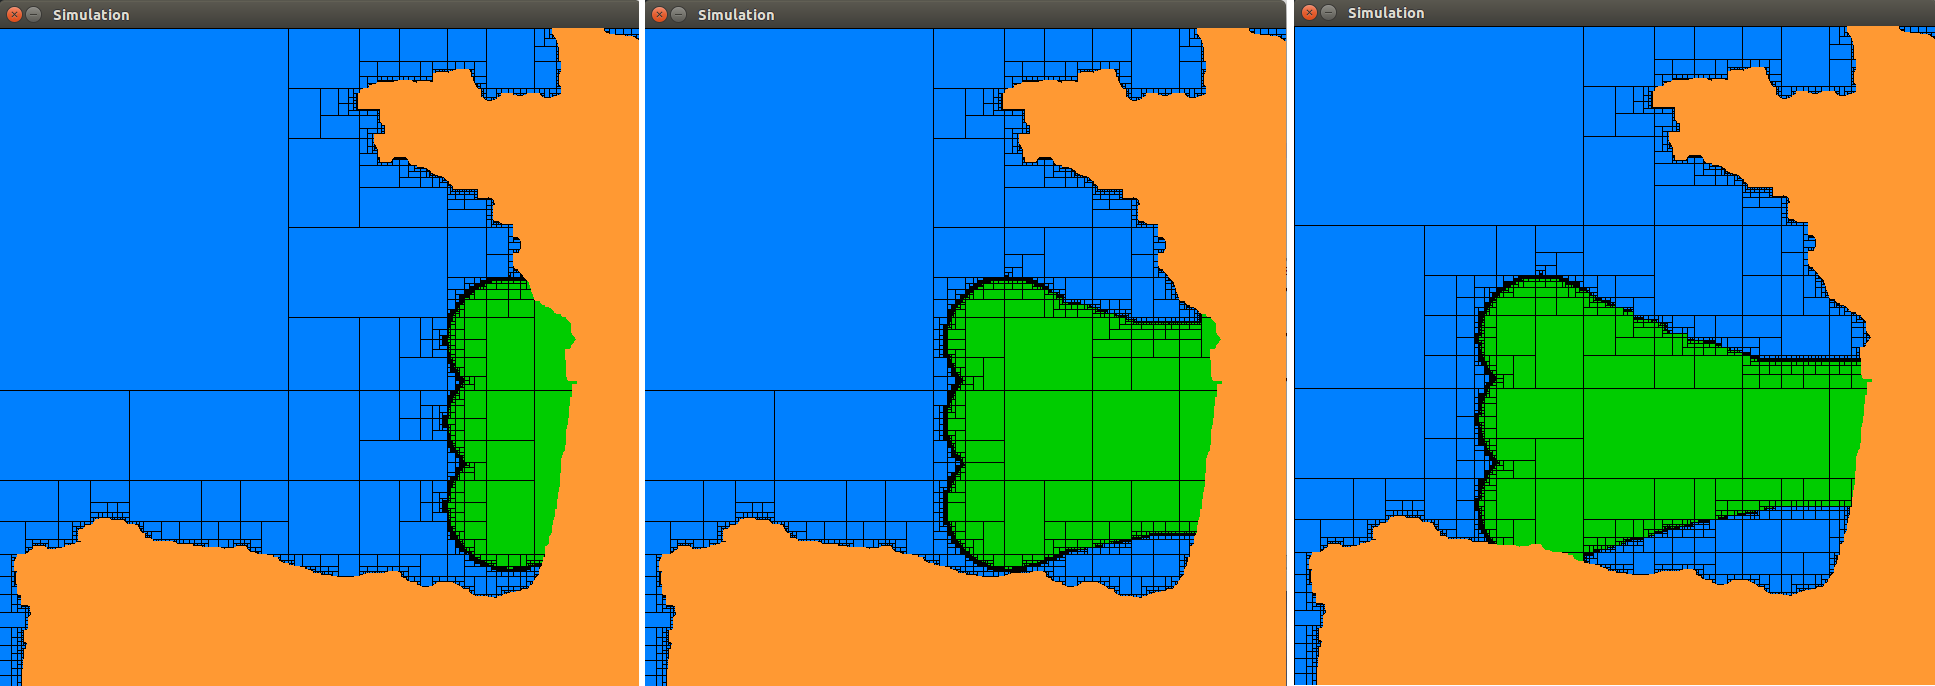
\includegraphics[scale=0.45]{SimulationFusion.png} 
    	\caption{Paving of the intersection between the Gascogne Golf, the robots and their erosion } 
    \label{S1 U S2}
	\end{figure} 
	
	
	
	
	

\end{document}
